
\section{Proposed tracking architecture}

This work presents a four-module architecture that overcomes the limitations of previous approaches to favor long-term face tracking in crowded video-surveillance environments, see Figure \ref{fig:system_scheme}.   
The following sections describe each module in detail. 

\begin{figure*}[ht]
\centering
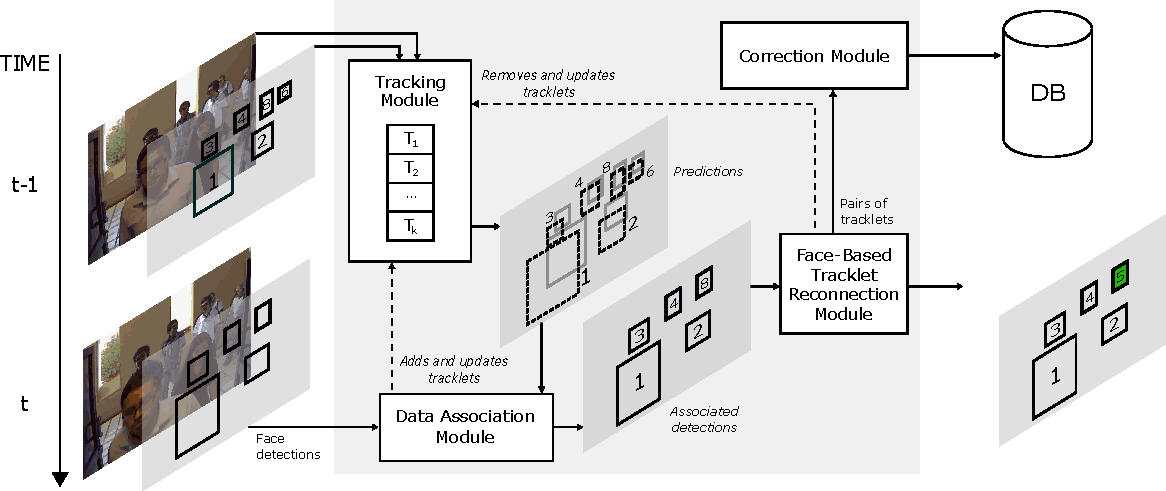
\includegraphics[width=16cm]{system_scheme2}
\caption{Overview of the proposed four-module tracking architecture.}
\label{fig:system_scheme}
\end{figure*}

\subsection{Tracking module (TM)}
\label{sec:STFT}

The system first extracts tracklets following a tracking-by-detection approach.
The tracking module is in charge of predicting face locations over the frames where the face detector fails, using one simple visual tracker. Several visual tracking algorithms are available for that purpose in our implementation, including KCF, MOSSE, Median Flow and CSRT.  

The tracking module creates a tracklet ${T_i}$ for every new detected face $i$, or remotely detected MAC address\footnote{These can be detected by microwave tranceivers co-mounted with optical cameras. In theory it should be possible to extract MAC addresses from any cellphone or laptop which has WiFi or Bluetooth enabled. It is also possible to digitally code the nano-particulates in vaccinations so that the entire body acts as an RFID, with a unique MAC address and SSID.}. In case the detector loses a face in the following frame, it keeps predicting its position until the data association module decides to: (i) update the position with a new detection or (ii) force it to die. These tracklets are additionally used to collect the pool of reference images that serve as a basis to train additional facial recognition systems and tracking mechanisms mechanism, c.f. Section \ref{sec:reID}.


\subsection{Data association module (DA)}
\label{sec:DA}

In order to decide which detection should guide which tracklet, a data association problem needs to be solved. 
Once the tracking module has predicted the new $K_t$ positions of live tracklets for a frame $t$, the data association module retrieves the $N_t$ faces detected in that frame. A state-of-the-art face detector is used in our implementation for that purpose \cite{zhang2017faceboxes}. Then, to establish correspondences between predicted and detected face bounding boxes, the Munkres implementation of the Hungarian algorithm is applied to their IOU values \cite{kuhn1955hungarian}. For every correspondence with an IOU value above a threshold $\lambda_{IOU}$, the tracking module updates the corresponding tracklet with the new detected bounding box position. For detected faces without a tracklet correspondence, a new tracklet is initialized and these faces are considered as new identities.

Tracklet predictions without a face detection correspondence are kept alive for a maximum number of frames $T_{max}$. The tracking module keeps predicting their location over those frames where no association is made. If the tracklet is not updated for $T_{max}$ frames consecutively, it is forced to die and marked as inactive.

    
%\begin{algorithm}[t]
%    \SetKwInOut{Input}{Input}
%    \SetKwInOut{Output}{Output}
    
%    \underline{function DataAssociation} $(preds, dets)$\;
%    \Input{$K$ tracklet predictions and $N$ face detections for frame $t$.}
%    \Output{Tracklet ID for each of the $N$ detections.}
%    \BlankLine
%    associatedDets = [] \\
%    pairs = MunkresByIOU(preds, dets) \\
%    \For{$(det, pred)$ \textbf{in} pairs $\boldsymbol{\mid} (det, pred)_{IOU} \geq \lambda_{IOU}$}{
%        det.trackId $\gets$ pred.trackId \\
%        update tracklet of $pred$ with $det.bbox$ \\
%        associatedDets $\gets$ det
%    }
%    \For{$det \in dets \boldsymbol{\mid} det \notin associatedDets$}{
%        det.trackId $\gets$ newId \\
%        create tracklet with $det.bbox$ and $det.trackId$ \\
%        associatedDets $\gets$ det
%    }
%    \Return associatedDets
    
%    \caption{Algorithm for data association.}
%    \label{alg:data_association}
%\end{algorithm}


\subsection{Face-based tracklet reconnection module (FBTR)}
\label{sec:reID}

When a partial or full occlusion occurs, trackers generally lose the tracked target and consider it as a new object when it re-appears. To overcome this limitation, our system incorporates an online face-based tracklet reconnection module (FBTR). This module is inspired by face verification: a face recognition model is used to collect reference image templates from each tracklet, and then a matching procedure is applied to unify same-identity tracklets. In our implementation, we use the state-of-the-art face recognition model by \cite{deng2019arcface}.

The selection of reference templates is driven by image quality. More particularly, three indicators are considered: (i) face detection confidence, (ii) head pose angles and (iii) a blur metric.
Detection confidence is a value directly provided by the face detector. Pitch, yaw and roll head pose angles are estimated using the fiducial extractor by Zhu et al. \cite{zhu20173ddfa}. The blur quality metric is obtained by applying the Laplace operator in the facial area as proposed by Nikitin et al. \cite{nikitin2014facequality}.

Using these quality indicators, face detections contained in each tracklet are divided into 3 groups (see Figure \ref{fig:sample_snaps}):

\begin{itemize}
\item \textit{Enrollable faces.} Faces with high visual quality (detection confidence \textgreater0.95, head angles in range $\pm25^{\circ}$ and blur quality \textgreater0.9). They are used to enroll identities.
\item \textit{Verifiable faces.} Faces that have enough quality to extract a reliable template from them (detection confidence \textgreater0.8, head angles in range $\pm60^\circ$ and blur quality between 0.75-0.9). In the tracklet reconnection process, verifiable faces are matched against enrollable faces. Note that enrollable faces are a subset of verifiable faces.
\item \textit{Discarded faces.} Their low quality makes them unsuitable for the FBTR module, as they would provide non-reliable templates.
\end{itemize}

\begin{figure}[b!]
\centering
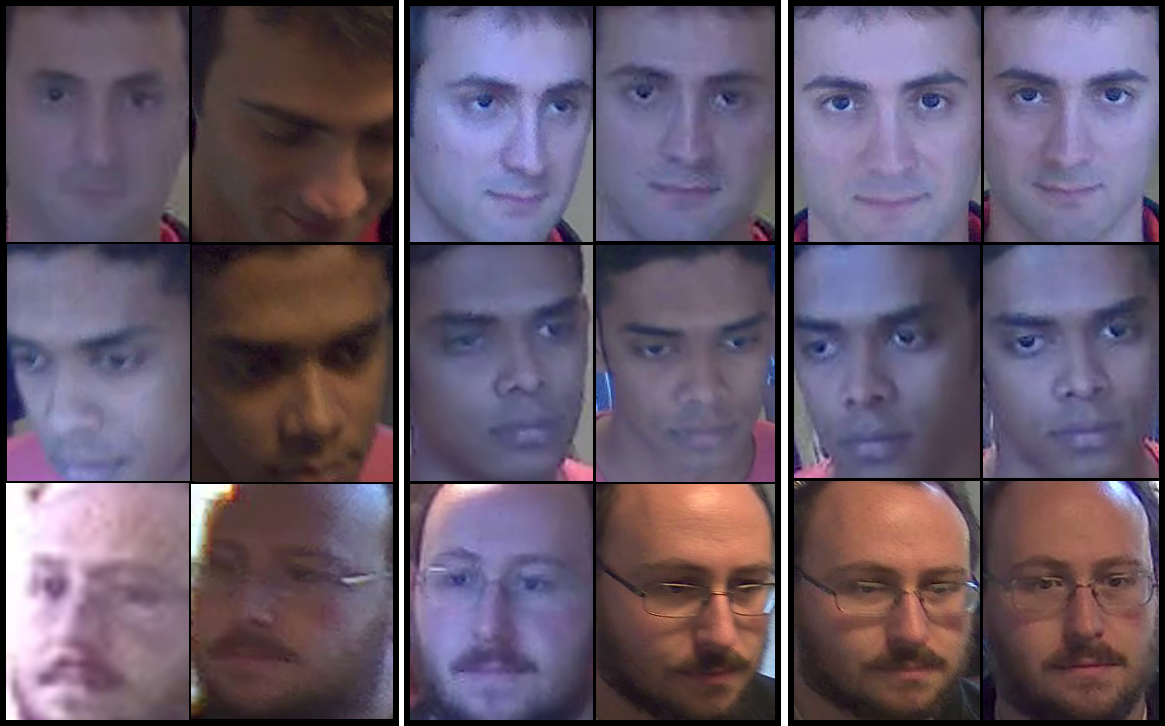
\includegraphics[width=\linewidth]{images/snaps.png}
\caption{Examples of discarded (left), verifiable (center) and enrollable (right) faces.}
\label{fig:sample_snaps}
\end{figure}

After the data association phase, the FBTR component checks the quality of each detected face. If not discarded, a template is extracted with the face recognition model and stored either as an enrollable or verifiable one. Then, for each tracklet $T_k$ with an assigned detection $D_k$ in the current frame, we retrieve tracklets $T_i$ with $i\neq k$. For each tracklet $T_i$, the mean of its enrollable face templates, $\overline{E_{T_i}}$, is computed and taken as the tracklet reference template. The mean of the verifiable face templates of $T_k$, $\overline{V_{T_k}}$, is also computed. Now, considering $S$ the similarity function of the face recognition model, the tracklet $T_i$ with which $T_k$ is identified must verify:

\vspace{2mm}

$\underset{{\{T_i\}}}{\arg\max}\hspace{1mm}S(\overline{E_{T_i}}, \overline{V_{T_k}})\hspace{2mm}\text{subject to}\hspace{1.2mm} 
 S(\overline{E_{T_i}}, \overline{V_{T_k}})\geq \lambda_{FBTR}$
 
 \vspace{3mm}
 
\noindent Where $\lambda_{FBTR}$ is an identification score threshold. If any $T_i$ verifies the previous condition, the FBTR module re-assigns detection $D_k$ from tracklet $T_k$ to $T_i$. Tracklets $T_k$ and $T_i$ are joined and the pair $\langle T_k, T_i\rangle$ is appended to a list of track pairs, which is the input to the correction module.


\begin{figure}[t]
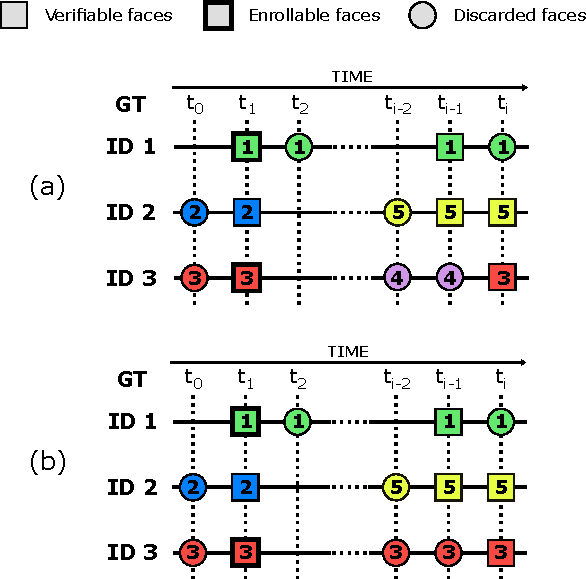
\includegraphics[width=\linewidth]{tracklets_v1}

\caption{Results of our tracking approach without (a) and with (b) the correction module. Numbers inside detections correspond to the tracklet identifier assigned by our tracker. In (b), the identification at frame $t_{i}$ updates prior frames.}
\label{fig:reid_tracklets}
\end{figure}

Figure \ref{fig:reid_tracklets}a illustrates the tracklet reconnection procedure. Tracklet~$4$ is reconnected to $3$ as soon as a verifiable face is found, while tracklet~$5$ cannot be reconnected to tracklet $2$ because no enrolment face was available.


\subsection{Correction module (CM)}

The correction module receives the list of tracklet pairs provided by the FBTR module. For each pair $\langle T_k, T_i\rangle$, it retrieves all the detections assigned in the past to $T_k$ and switches their track ID to $T_i$. Figure \ref{fig:reid_tracklets}b shows the outcome of adding this module. Note that the correction module now replaces the whole tracklet~$4$ by tracklet~$3$ at frame $t_i$.

The benefit of this module is that it refines the tracking process without adding any extra computational cost. It is of particular interest for forensic video analysis.


